\documentclass[twoside]{book}

% Packages required by doxygen
\usepackage{calc}
\usepackage{doxygen}
\usepackage{graphicx}
\usepackage[utf8]{inputenc}
\usepackage{makeidx}
\usepackage{multicol}
\usepackage{multirow}
\usepackage{fixltx2e}
\PassOptionsToPackage{warn}{textcomp}
\usepackage{textcomp}
\usepackage[nointegrals]{wasysym}
\usepackage[table]{xcolor}

% Font selection
\usepackage[T1]{fontenc}
\usepackage{mathptmx}
\usepackage[scaled=.90]{helvet}
\usepackage{courier}
\usepackage{amssymb}
\usepackage{sectsty}
\renewcommand{\familydefault}{\sfdefault}
\allsectionsfont{%
  \fontseries{bc}\selectfont%
  \color{darkgray}%
}
\renewcommand{\DoxyLabelFont}{%
  \fontseries{bc}\selectfont%
  \color{darkgray}%
}
\newcommand{\+}{\discretionary{\mbox{\scriptsize$\hookleftarrow$}}{}{}}

% Page & text layout
\usepackage{geometry}
\geometry{%
  a4paper,%
  top=2.5cm,%
  bottom=2.5cm,%
  left=2.5cm,%
  right=2.5cm%
}
\tolerance=750
\hfuzz=15pt
\hbadness=750
\setlength{\emergencystretch}{15pt}
\setlength{\parindent}{0cm}
\setlength{\parskip}{0.2cm}
\makeatletter
\renewcommand{\paragraph}{%
  \@startsection{paragraph}{4}{0ex}{-1.0ex}{1.0ex}{%
    \normalfont\normalsize\bfseries\SS@parafont%
  }%
}
\renewcommand{\subparagraph}{%
  \@startsection{subparagraph}{5}{0ex}{-1.0ex}{1.0ex}{%
    \normalfont\normalsize\bfseries\SS@subparafont%
  }%
}
\makeatother

% Headers & footers
\usepackage{fancyhdr}
\pagestyle{fancyplain}
\fancyhead[LE]{\fancyplain{}{\bfseries\thepage}}
\fancyhead[CE]{\fancyplain{}{}}
\fancyhead[RE]{\fancyplain{}{\bfseries\leftmark}}
\fancyhead[LO]{\fancyplain{}{\bfseries\rightmark}}
\fancyhead[CO]{\fancyplain{}{}}
\fancyhead[RO]{\fancyplain{}{\bfseries\thepage}}
\fancyfoot[LE]{\fancyplain{}{}}
\fancyfoot[CE]{\fancyplain{}{}}
\fancyfoot[RE]{\fancyplain{}{\bfseries\scriptsize Generated on Sun May 25 2014 21\+:43\+:22 for Manchot by Doxygen }}
\fancyfoot[LO]{\fancyplain{}{\bfseries\scriptsize Generated on Sun May 25 2014 21\+:43\+:22 for Manchot by Doxygen }}
\fancyfoot[CO]{\fancyplain{}{}}
\fancyfoot[RO]{\fancyplain{}{}}
\renewcommand{\footrulewidth}{0.4pt}
\renewcommand{\chaptermark}[1]{%
  \markboth{#1}{}%
}
\renewcommand{\sectionmark}[1]{%
  \markright{\thesection\ #1}%
}

% Indices & bibliography
\usepackage{natbib}
\usepackage[titles]{tocloft}
\setcounter{tocdepth}{3}
\setcounter{secnumdepth}{5}
\makeindex

% Hyperlinks (required, but should be loaded last)
\usepackage{ifpdf}
\ifpdf
  \usepackage[pdftex,pagebackref=true]{hyperref}
\else
  \usepackage[ps2pdf,pagebackref=true]{hyperref}
\fi
\hypersetup{%
  colorlinks=true,%
  linkcolor=blue,%
  citecolor=blue,%
  unicode%
}

% Custom commands
\newcommand{\clearemptydoublepage}{%
  \newpage{\pagestyle{empty}\cleardoublepage}%
}


%===== C O N T E N T S =====

\begin{document}

% Titlepage & ToC
\hypersetup{pageanchor=false,
             bookmarks=true,
             bookmarksnumbered=true,
             pdfencoding=unicode
            }
\pagenumbering{roman}
\begin{titlepage}
\vspace*{7cm}
\begin{center}%
{\Large Manchot }\\
\vspace*{1cm}
{\large Generated by Doxygen 1.8.7}\\
\vspace*{0.5cm}
{\small Sun May 25 2014 21:43:22}\\
\end{center}
\end{titlepage}
\clearemptydoublepage
\tableofcontents
\clearemptydoublepage
\pagenumbering{arabic}
\hypersetup{pageanchor=true}

%--- Begin generated contents ---
\chapter{Namespace Index}
\section{Packages}
Here are the packages with brief descriptions (if available)\+:\begin{DoxyCompactList}
\item\contentsline{section}{\hyperlink{namespace_manchot}{Manchot} }{\pageref{namespace_manchot}}{}
\item\contentsline{section}{\hyperlink{namespace_manchot_1_1_properties}{Manchot.\+Properties} }{\pageref{namespace_manchot_1_1_properties}}{}
\end{DoxyCompactList}

\chapter{Hierarchical Index}
\section{Class Hierarchy}
This inheritance list is sorted roughly, but not completely, alphabetically\+:\begin{DoxyCompactList}
\item \contentsline{section}{Manchot.\+Evenement}{\pageref{class_manchot_1_1_evenement}}{}
\item Form\begin{DoxyCompactList}
\item \contentsline{section}{Manchot.\+Form1}{\pageref{class_manchot_1_1_form1}}{}
\end{DoxyCompactList}
\item \contentsline{section}{Manchot.\+Traitement}{\pageref{class_manchot_1_1_traitement}}{}
\end{DoxyCompactList}

\chapter{Class Index}
\section{Class List}
Here are the classes, structs, unions and interfaces with brief descriptions\+:\begin{DoxyCompactList}
\item\contentsline{section}{\hyperlink{class_manchot_1_1_evenement}{Manchot.\+Evenement} }{\pageref{class_manchot_1_1_evenement}}{}
\item\contentsline{section}{\hyperlink{class_manchot_1_1_form1}{Manchot.\+Form1} }{\pageref{class_manchot_1_1_form1}}{}
\item\contentsline{section}{\hyperlink{class_manchot_1_1_traitement}{Manchot.\+Traitement} }{\pageref{class_manchot_1_1_traitement}}{}
\end{DoxyCompactList}

\chapter{Namespace Documentation}
\hypertarget{namespace_manchot}{\section{Package Manchot}
\label{namespace_manchot}\index{Manchot@{Manchot}}
}
\subsection*{Namespaces}
\begin{DoxyCompactItemize}
\item 
package \hyperlink{namespace_manchot_1_1_properties}{Properties}
\end{DoxyCompactItemize}
\subsection*{Classes}
\begin{DoxyCompactItemize}
\item 
class \hyperlink{class_manchot_1_1_evenement}{Evenement}
\item 
class \hyperlink{class_manchot_1_1_form1}{Form1}
\item 
class {\bfseries Program}
\item 
class \hyperlink{class_manchot_1_1_traitement}{Traitement}
\end{DoxyCompactItemize}

\hypertarget{namespace_manchot_1_1_properties}{\section{Package Manchot.\+Properties}
\label{namespace_manchot_1_1_properties}\index{Manchot.\+Properties@{Manchot.\+Properties}}
}
\subsection*{Classes}
\begin{DoxyCompactItemize}
\item 
class {\bfseries Resources}
\begin{DoxyCompactList}\small\item\em A strongly-\/typed resource class, for looking up localized strings, etc. \end{DoxyCompactList}\item 
class {\bfseries Settings}
\end{DoxyCompactItemize}

\chapter{Class Documentation}
\hypertarget{class_manchot_1_1_evenement}{\section{Manchot.\+Evenement Class Reference}
\label{class_manchot_1_1_evenement}\index{Manchot.\+Evenement@{Manchot.\+Evenement}}
}
\subsection*{Public Member Functions}
\begin{DoxyCompactItemize}
\item 
\hypertarget{class_manchot_1_1_evenement_a34158d2e84e6c90e0d5aaa41da97c06c}{{\bfseries Evenement} (double abs\+Debut, Date\+Time debut\+Date)}\label{class_manchot_1_1_evenement_a34158d2e84e6c90e0d5aaa41da97c06c}

\item 
void \hyperlink{class_manchot_1_1_evenement_a16500af63cab5260508f510b2c4ab63e}{analyser} (Double\mbox{[}$\,$\mbox{]} data)
\begin{DoxyCompactList}\small\item\em L'algorihtme d'analyse de détection des cas simples \end{DoxyCompactList}\item 
\hypertarget{class_manchot_1_1_evenement_add7952e30aa5b337001eec03281e1515}{void {\bfseries to\+String} ()}\label{class_manchot_1_1_evenement_add7952e30aa5b337001eec03281e1515}

\end{DoxyCompactItemize}
\subsection*{Public Attributes}
\begin{DoxyCompactItemize}
\item 
\hypertarget{class_manchot_1_1_evenement_aa91230c351cec120029e1be48361c1f9}{double {\bfseries abs\+Debut}}\label{class_manchot_1_1_evenement_aa91230c351cec120029e1be48361c1f9}

\item 
\hypertarget{class_manchot_1_1_evenement_a76aac7ad1749ec34ce6b4d0cc45c6719}{double {\bfseries abs\+Fin}}\label{class_manchot_1_1_evenement_a76aac7ad1749ec34ce6b4d0cc45c6719}

\item 
\hypertarget{class_manchot_1_1_evenement_a9a465017ad41a4cd246887a2575207e1}{Date\+Time {\bfseries date\+Debut}}\label{class_manchot_1_1_evenement_a9a465017ad41a4cd246887a2575207e1}

\item 
\hypertarget{class_manchot_1_1_evenement_a2e8354a25ea824281aa00ce6e75bf36d}{string {\bfseries heure}}\label{class_manchot_1_1_evenement_a2e8354a25ea824281aa00ce6e75bf36d}

\item 
\hypertarget{class_manchot_1_1_evenement_a830974e04282d744b6c3b62101601208}{string {\bfseries analyse}}\label{class_manchot_1_1_evenement_a830974e04282d744b6c3b62101601208}

\end{DoxyCompactItemize}


\subsection{Member Function Documentation}
\hypertarget{class_manchot_1_1_evenement_a16500af63cab5260508f510b2c4ab63e}{\index{Manchot\+::\+Evenement@{Manchot\+::\+Evenement}!analyser@{analyser}}
\index{analyser@{analyser}!Manchot\+::\+Evenement@{Manchot\+::\+Evenement}}
\subsubsection[{analyser}]{\setlength{\rightskip}{0pt plus 5cm}void Manchot.\+Evenement.\+analyser (
\begin{DoxyParamCaption}
\item[{Double\mbox{[}$\,$\mbox{]}}]{data}
\end{DoxyParamCaption}
)}}\label{class_manchot_1_1_evenement_a16500af63cab5260508f510b2c4ab63e}


L'algorihtme d'analyse de détection des cas simples 


\begin{DoxyParams}{Parameters}
{\em data} & Tableau de Double contenant les données\\
\hline
\end{DoxyParams}


The documentation for this class was generated from the following file\+:\begin{DoxyCompactItemize}
\item 
C\+:/\+Users/\+Kévin/\+Documents/\+Git\+Hub/projet/\+Manchot/\+Manchot/Evenement.\+cs\end{DoxyCompactItemize}

\hypertarget{class_manchot_1_1_form1}{\section{Manchot.\+Form1 Class Reference}
\label{class_manchot_1_1_form1}\index{Manchot.\+Form1@{Manchot.\+Form1}}
}
Inheritance diagram for Manchot.\+Form1\+:\begin{figure}[H]
\begin{center}
\leavevmode
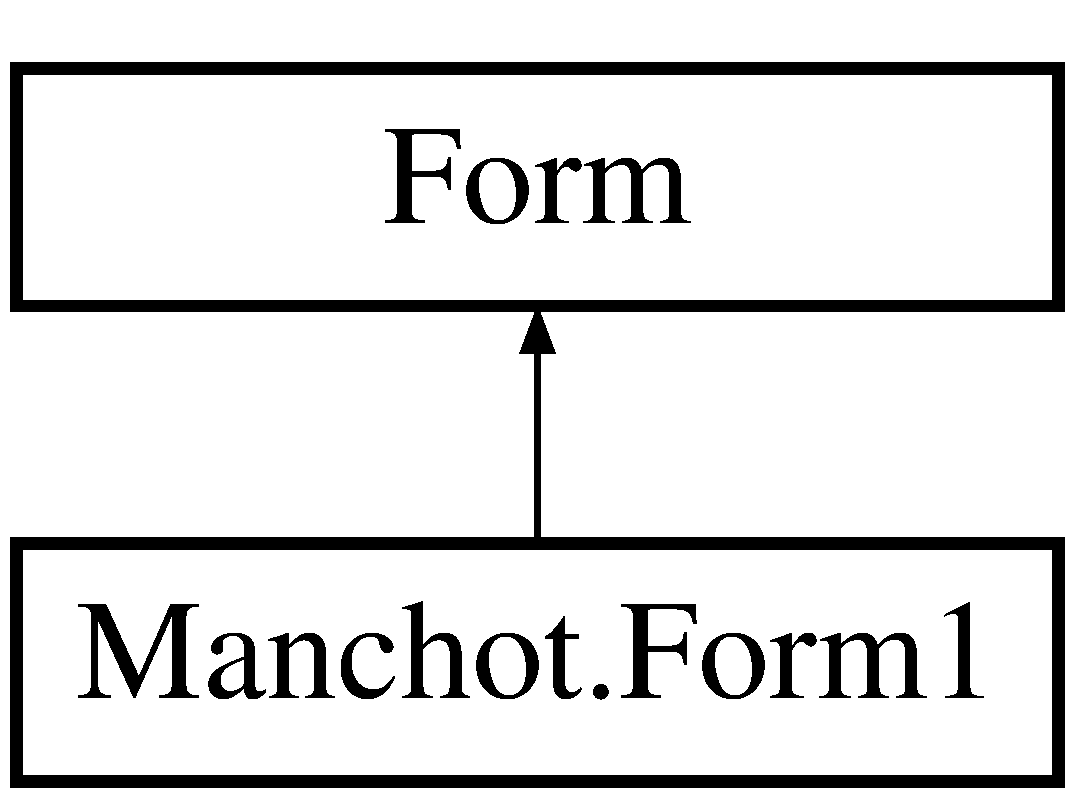
\includegraphics[height=2.000000cm]{class_manchot_1_1_form1}
\end{center}
\end{figure}
\subsection*{Public Member Functions}
\begin{DoxyCompactItemize}
\item 
\hypertarget{class_manchot_1_1_form1_aa25ebfdd6474a11a841d1cd8a1975e68}{void {\bfseries Message\+Flash} (Object message)}\label{class_manchot_1_1_form1_aa25ebfdd6474a11a841d1cd8a1975e68}

\end{DoxyCompactItemize}
\subsection*{Protected Member Functions}
\begin{DoxyCompactItemize}
\item 
override void \hyperlink{class_manchot_1_1_form1_a42b58d107e6bbcc4c30174be175bcc37}{Dispose} (bool disposing)
\begin{DoxyCompactList}\small\item\em Clean up any resources being used. \end{DoxyCompactList}\end{DoxyCompactItemize}


\subsection{Member Function Documentation}
\hypertarget{class_manchot_1_1_form1_a42b58d107e6bbcc4c30174be175bcc37}{\index{Manchot\+::\+Form1@{Manchot\+::\+Form1}!Dispose@{Dispose}}
\index{Dispose@{Dispose}!Manchot\+::\+Form1@{Manchot\+::\+Form1}}
\subsubsection[{Dispose}]{\setlength{\rightskip}{0pt plus 5cm}override void Manchot.\+Form1.\+Dispose (
\begin{DoxyParamCaption}
\item[{bool}]{disposing}
\end{DoxyParamCaption}
)\hspace{0.3cm}{\ttfamily [protected]}}}\label{class_manchot_1_1_form1_a42b58d107e6bbcc4c30174be175bcc37}


Clean up any resources being used. 


\begin{DoxyParams}{Parameters}
{\em disposing} & true if managed resources should be disposed; otherwise, false.\\
\hline
\end{DoxyParams}


The documentation for this class was generated from the following files\+:\begin{DoxyCompactItemize}
\item 
C\+:/\+Users/\+Kévin/\+Documents/\+Git\+Hub/projet/\+Manchot/\+Manchot/Form1.\+cs\item 
C\+:/\+Users/\+Kévin/\+Documents/\+Git\+Hub/projet/\+Manchot/\+Manchot/Form1.\+Designer.\+cs\end{DoxyCompactItemize}

\hypertarget{class_manchot_1_1_traitement}{\section{Manchot.\+Traitement Class Reference}
\label{class_manchot_1_1_traitement}\index{Manchot.\+Traitement@{Manchot.\+Traitement}}
}
\subsection*{Static Public Member Functions}
\begin{DoxyCompactItemize}
\item 
static double\mbox{[}$\,$\mbox{]}\mbox{[}$\,$\mbox{]} \hyperlink{class_manchot_1_1_traitement_afedd59a6201aa10f4c57d332efd86407}{supression\+Bruit} (double\mbox{[}$\,$\mbox{]}\mbox{[}$\,$\mbox{]} measured\+Data)
\begin{DoxyCompactList}\small\item\em Fonction permettant de supprimer le bruit proche de 0 \+: Lorsqu'une valeur est inferieur à 0.\+5, la met à 0 \end{DoxyCompactList}\item 
static double\mbox{[}$\,$\mbox{]}\mbox{[}$\,$\mbox{]} \hyperlink{class_manchot_1_1_traitement_aa0d655f8bef3619bdfc36ea4fd47d6e7}{filtre\+Moyenne} (double\mbox{[}$\,$\mbox{]}\mbox{[}$\,$\mbox{]} measure\+Data)
\begin{DoxyCompactList}\small\item\em Fonction de filtrage \+: permet de lisser la courbe en utilisant un algorithme de filtre moyenneur. Chaque valeur et la moyenne de la valeur la précédente et la valeur la succédant \end{DoxyCompactList}\item 
\hypertarget{class_manchot_1_1_traitement_a59f8016b30fb1b50dd4e1c59db6854b1}{static double {\bfseries median} (double\mbox{[}$\,$\mbox{]} arr)}\label{class_manchot_1_1_traitement_a59f8016b30fb1b50dd4e1c59db6854b1}

\item 
\hypertarget{class_manchot_1_1_traitement_aed43f620f20d15a68db0f31ef11e7b78}{static double\mbox{[}$\,$\mbox{]} {\bfseries filtre\+Median} (double\mbox{[}$\,$\mbox{]} arr, double wl)}\label{class_manchot_1_1_traitement_aed43f620f20d15a68db0f31ef11e7b78}

\item 
\hypertarget{class_manchot_1_1_traitement_a36afab1b1bb57a7bc320d761c7654cda}{static double {\bfseries pourcentage\+Bruit} (double\mbox{[}$\,$\mbox{]}\mbox{[}$\,$\mbox{]} measured\+Data)}\label{class_manchot_1_1_traitement_a36afab1b1bb57a7bc320d761c7654cda}

\item 
static \hyperlink{class_manchot_1_1_evenement}{Evenement} \hyperlink{class_manchot_1_1_traitement_aa07e00505b10ae01c11fcfa6d62da67f}{date\+Evenement} (Date\+Time date, double abscisse)
\end{DoxyCompactItemize}


\subsection{Member Function Documentation}
\hypertarget{class_manchot_1_1_traitement_aa07e00505b10ae01c11fcfa6d62da67f}{\index{Manchot\+::\+Traitement@{Manchot\+::\+Traitement}!date\+Evenement@{date\+Evenement}}
\index{date\+Evenement@{date\+Evenement}!Manchot\+::\+Traitement@{Manchot\+::\+Traitement}}
\subsubsection[{date\+Evenement}]{\setlength{\rightskip}{0pt plus 5cm}static {\bf Evenement} Manchot.\+Traitement.\+date\+Evenement (
\begin{DoxyParamCaption}
\item[{Date\+Time}]{date, }
\item[{double}]{abscisse}
\end{DoxyParamCaption}
)\hspace{0.3cm}{\ttfamily [static]}}}\label{class_manchot_1_1_traitement_aa07e00505b10ae01c11fcfa6d62da67f}
Calcule la date (heure et secondes) d'un évenement grâce à la correspondance entre l'abscisse du début de l'évement et les métadonnées du fichier. \hypertarget{class_manchot_1_1_traitement_aa0d655f8bef3619bdfc36ea4fd47d6e7}{\index{Manchot\+::\+Traitement@{Manchot\+::\+Traitement}!filtre\+Moyenne@{filtre\+Moyenne}}
\index{filtre\+Moyenne@{filtre\+Moyenne}!Manchot\+::\+Traitement@{Manchot\+::\+Traitement}}
\subsubsection[{filtre\+Moyenne}]{\setlength{\rightskip}{0pt plus 5cm}static double \mbox{[}$\,$\mbox{]}\mbox{[}$\,$\mbox{]} Manchot.\+Traitement.\+filtre\+Moyenne (
\begin{DoxyParamCaption}
\item[{double}]{measure\+Data\mbox{[}$\,$\mbox{]}\mbox{[}$\,$\mbox{]}}
\end{DoxyParamCaption}
)\hspace{0.3cm}{\ttfamily [static]}}}\label{class_manchot_1_1_traitement_aa0d655f8bef3619bdfc36ea4fd47d6e7}


Fonction de filtrage \+: permet de lisser la courbe en utilisant un algorithme de filtre moyenneur. Chaque valeur et la moyenne de la valeur la précédente et la valeur la succédant 


\begin{DoxyParams}{Parameters}
{\em measure\+Data} & \\
\hline
\end{DoxyParams}
\begin{DoxyReturn}{Returns}

\end{DoxyReturn}
\hypertarget{class_manchot_1_1_traitement_afedd59a6201aa10f4c57d332efd86407}{\index{Manchot\+::\+Traitement@{Manchot\+::\+Traitement}!supression\+Bruit@{supression\+Bruit}}
\index{supression\+Bruit@{supression\+Bruit}!Manchot\+::\+Traitement@{Manchot\+::\+Traitement}}
\subsubsection[{supression\+Bruit}]{\setlength{\rightskip}{0pt plus 5cm}static double \mbox{[}$\,$\mbox{]}\mbox{[}$\,$\mbox{]} Manchot.\+Traitement.\+supression\+Bruit (
\begin{DoxyParamCaption}
\item[{double}]{measured\+Data\mbox{[}$\,$\mbox{]}\mbox{[}$\,$\mbox{]}}
\end{DoxyParamCaption}
)\hspace{0.3cm}{\ttfamily [static]}}}\label{class_manchot_1_1_traitement_afedd59a6201aa10f4c57d332efd86407}


Fonction permettant de supprimer le bruit proche de 0 \+: Lorsqu'une valeur est inferieur à 0.\+5, la met à 0 


\begin{DoxyParams}{Parameters}
{\em measured\+Data} & \\
\hline
\end{DoxyParams}
\begin{DoxyReturn}{Returns}

\end{DoxyReturn}


The documentation for this class was generated from the following file\+:\begin{DoxyCompactItemize}
\item 
C\+:/\+Users/\+Kévin/\+Documents/\+Git\+Hub/projet/\+Manchot/\+Manchot/Traitement.\+cs\end{DoxyCompactItemize}

%--- End generated contents ---

% Index
\newpage
\phantomsection
\addcontentsline{toc}{chapter}{Index}
\printindex

\end{document}
